\documentclass[fleqn,10pt]{wlscirep}
\title{Survey on Surface Parameterization}

\author[1,*]{Xuan Li}
\affil[1]{Department of Computer Science, Stony Brook University}
\affil[*]{SBU ID: 111676019}

\newtheorem{definition}{Definition}[section]
\newtheorem{theorem}{Theorem}[section]
\newtheorem{corollary}{Corollary}[theorem]
\newtheorem{lemma}[theorem]{Lemma}


\usepackage{graphicx}
\usepackage{caption}
\usepackage{subcaption}

%\keywords{Keyword1, Keyword2, Keyword3}

\begin{abstract}
This paper review mainly includes four papers: \cite{Gortler:2006:DOM:1133946.1648437} \cite{Aigerman:2015:OTE:2816795.2818099}( I will also review the main ideas of \cite{Aigerman:2016:HOT:2980179.2982412}\cite{Aigerman:2017:SOT:3072959.3073615}, which are from the same geometry theory as \cite{Aigerman:2015:OTE:2816795.2818099}) \cite{Bright:2017:HGP:3072959.3073646}\cite{1704.06873}. \cite{Gortler:2006:DOM:1133946.1648437} studied discrete one-forms on meshes. Gortler proved the discrete version of Poincar\'e–Hopf index theorem. He  used index theorem to give a simple proof of Tutte's embedding theorem and made some kind of generalization of Tutte's embedding theorem. \cite{Aigerman:2015:OTE:2816795.2818099} used Euclidean orbifold structures to apply Tutte's embedding algorithm to sphere-type meshes. Besides, \cite{Aigerman:2016:HOT:2980179.2982412}\cite{Aigerman:2017:SOT:3072959.3073615} generalized this idea to hyperbolic orbifolds and spherical orbifold. \cite{Bright:2017:HGP:3072959.3073646} generalized the idea of orbifolds, allowing the rotation angles of singularities not to satisfy the requirements of orbifolds. This method used some convexification technique to convexify the optimization problem, which appered in \cite{Lipman:2012:BDM:2185520.2185604}\cite{Chen:2015:BDH:2809654.2766989}.
\cite{Aigerman:2015:OTE:2816795.2818099} claimed that under the constraint of orbifold, orbifold Tutte embeddings approximate conformal maps. So this actually gives a linear method to compute conformal maps. \cite{1704.06873} also proposed a linear method, but under the view of differential geometry and PDE (i.e. Poisson equation). The solution to a Poisson equation is determined by its boundary data. So the method is about how to get boundary data and how to extend the boundary data conformally into the interior. Interestingly, BFF can also solve global paramerization of cone surfaces.
\end{abstract}
\begin{document}

\flushbottom
\maketitle
% * <john.hammersley@gmail.com> 2015-02-09T12:07:31.197Z:
%
%  Click the title above to edit the author information and abstract
%

\section{Discrete one-forms on meshes and applications to 3D mesh parameterization}

In this section, we review the paper \cite{Gortler:2006:DOM:1133946.1648437}. It is the theoretical foundation of \cite{Aigerman:2015:OTE:2816795.2818099}\cite{Bright:2017:HGP:3072959.3073646}.

\subsection{Tutte Graph Embedding}

In 1963, Tutte proved his celebrated “spring embedding” theorem for planar graphs:
\begin{theorem}\label{tutte-theorem}
Let $G = \left<V , E , F \right>$ be a 3-connected planar graph with boundary vertices $B \subset V$ defining a unique unbounded exterior face $f_e$ . Suppose $\partial f_e$ is embedded in the plane as a (not necessarily strictly) convex planar polygon, and each interior vertex is positioned in the plane as a strictly convex combination of its neighbors, then the straight-line drawing of $G$ with these vertex positions is an embedding. In addition, this embedding has strictly convex interior faces.
\end{theorem}
As we know, surface meshes are 3-connected, so this theorem is very important for parameterization. It lead to bijective parameterizations of surface meshes.

Tutte used the following linear system to get the 2D embedding of graph:
\begin{equation}
\begin{split}
\sum_{v_j \in \mathit{N}(v_i)} w_{ij}x_j &= x_i, i = 1, ..., |V - B|\\
\sum_{v_j \in \mathit{N}(v_i)} w_{ij}y_j &= y_i, i = 1, ..., |V - B|\\
x_i &= b_i^x, i = |V-B| + 1, ... , |V|\\
y_i &= b_i^y, i = |V-B| + 1, ... , |V|
\end{split}
\end{equation}
where $\sum_{j}w_{ij} = 1, \forall v_i$, and $w > 0$.


This system is full-rank, so has a unique solution. Tutte proved that the solution is an embedding of the graph. 

In this paper, Goltler used the properties of harmonic one-form to provide a simple and nice proof to this theorem.

\begin{definition}
A discrete one-form $[G, \Delta z]$ is an assignment of a real value $\Delta z_{uv}$ to each half edge $(u,v)$ of $G$ such that $\Delta z_{uv} =-\Delta z_{vu}$
\end{definition}

\begin{definition}
Given a set of (not necessarily symmetric) positive weights $w_h$ associated with each half
edge $h$ in G and a one-form $[G,  \Delta z]$, a vertex $v$ is called \textbf{co-closed} with respect to (wrt) $w$ if
$$\sum_{h\in \delta v}w_h \Delta z_h =0.$$
A face $f$ is called \textbf{closed} if
 $$\sum_{h\in \partial f}\Delta z_h = 0. $$
 A one-form whose faces are all closed and all vertices co-closed wrt some set of weights is called \textbf{harmonic}.
\end{definition}

\begin{definition}
Let $[G,  \Delta z]$ be a non-vanishing one-form. The \textbf{index of a vertex} $v$ in $[G,  \Delta z]$ is $ind(v) = (2 - sc(v))/2$, where $sc(v)$ is the number of sign changes in the values of  $\Delta z$ as one traverses the half-edges of $\delta v$ in order. The \textbf{index of a face} $f$ in $[G, z]$ is $ind(f) = (2 - sc(f))/2$, where $sc(f)$ is the number of sign changes in the values of  $\Delta z$ as one traverses the half edges of $\partial f$ in order. $v$ is called a \textbf{non-singular vertex} if $ind(v) = 0$ and a \textbf{saddle vertex if $ind(v) < 0$. If $ind(v) = 1$, and all values of } $\Delta z$ at $v$ are positive, $v$ is called a \textbf{source}, otherwise $v$ is called a \textbf{sink}. $f$ is called a \textbf{non-singular face} if $ind(f)=0$ and a \textbf{saddle face} if $ind(f)<0$ .If $ind(f)=1$, $f$ is called a \textbf{vortex}.
\end{definition}


Under this framework, the author proved the index theorem:
\begin{theorem}(Index Theorem)
If $G$ is a closed oriented manifold mesh of genus $g$, then any non-vanishing one-form $[G,  \Delta z]$ satisfies 
$$ \sum_{v\in V} ind(V) + \sum_{f\in F} ind(f)= 2 - 2g$$

\end{theorem}



Tutte's system can define a series of one-form:
define $z_i = \alpha x_i + \beta y_i$, then we define a one-form as $\Delta z_{ij} = -\Delta z_{ji} = z_j - z_i$. Tutte's system implies that every interior vertex $v$ of $[G,  \Delta z]$ is co-closed and every face is closed wrt $w$, so $[G,  \Delta z]$ is harmonic one-form.

The author proved Tutte's embedding theorem by index theorem and generalized it to cases of multiple non-convex boundaries, and even high genus meshes. 

But to apply index theorem, we need to view the focused mesh as a closed mesh. In the case of of multiple non-convex boundaries, we view it as a sphere-type mesh with punctures, which correspond to boundary components. Specifically, one puncture corresponds to the exterior face, called unbounded face and other punctures corresponds interior boudnaries, called bounded faces. That is, every boundary is a face.

In this point of view, the author proved the following key lemma:
\begin{lemma}
If $G$ has genus 0 and $[G,  z]$ is a non-vanishing one-form such that all $F$ faces are closed, $|V - B|$ vertices are co-closed wrt some set of positive weights and of the remaining $B$ vertices, $|B - 2|$ have index   0, then $[G,  z]$ has no saddle vertices and no saddle faces.
\end{lemma}



This lemma leads to Theorem \ref{tutte-theorem} by proving every interior vertex is a wheel:
\begin{definition}
Let $v$ be a vertex of $G$. Let $\alpha_i$ be the signed angles between adjacent half-edges in $\delta v$
(angles are measured by going the ``short" way between half edges, so $0 < |\alpha_i| < \pi$ ). $v$ is called a wheel vertex of $[G,x,y]$ if $\alpha_i$ all have the same sign and $|
\alpha_i|=2\pi$.
\end{definition}

\subsection{Multiple Non-convex Boundaries}

In the case of of multiple non-convex boundaries, still by index theorem, the auther proved:
\begin{lemma} \label{multi-boundary}
Suppose that: (1) $G$ is an oriented 3-connected mesh of genus 0 having multiple exterior faces. (2) The boundary of the unbounded face is mapped to the plane with positive edge lengths and turning number $2\pi$. (3) The boundaries of the bounded faces are mapped to the plane with positive edge lengths and turning number $-2\pi$. (4) $[G,x,y]$ is the straight line drawing of $G$ where each internal vertex is positioned as a convex combination of its neighbors. (5) In $[G,x,y]$ the reflex vertices of all of the exterior face boundaries are also in the convex hull of their neighbors. Then for any $\alpha, \beta$ and $[G,  \Delta z]$ constructed as in (4), no vertex or interior face is a saddle in $[G,  \Delta z]$.
\end{lemma}

This lead to the generalization of Tutte's theorem:
\begin{theorem}
Under the conditions of Lemma \ref{multi-boundary}, all interior faces of $[G,x,y]$ are convex and all interior vertices are wheels. Moreover, if all the exterior faces are embedded as disjoint simple polygons (edge crossings are not allowed), then all faces of $[G, x, y]$ are disjoint.
\end{theorem}

The setting of Lemma \ref{multi-boundary} allows non-convex boundary, but adds an extra constraint about reflex boundary-vertices, which makes this theorem not very practical in parameterization. But this provides an insight that the interior behavior is all determined by boundary faces. This insight was used in \cite{Bright:2017:HGP:3072959.3073646}.

\subsection{Global Parameterization}

For high genus surfaces, similar theorems exists. But one of understandings of global parameterization should be mentioned, which also appeared in \cite{Aigerman:2015:OTE:2816795.2818099}\cite{Bright:2017:HGP:3072959.3073646} \cite{1704.06873}.

Because of topological constraints, high-genus closed meshes cannot flatten into Euclidean plane directly. Instead, we need to cut the mesh $S$ into disk-type mesh $S_c$. $S_c$ can be viewed as a local chart of $S$. By parameterization, we can defined a pull-back metric $g_c$ on $S_c$ by $l(e) = |f(v_0) - f(v_1)|$ (This is the discrete version of Riemannian metric, which is determined by edge lengths satisfied triangle inequality). The global paramerterization means the metric $g_c$ of $S_c$ induces a global metric $g$ on $S$. The slice form a graph $G_c\subset S$, each edge $e$ of $G_c$ will be split into two copies $e_0$ and $e_1$, global metric means $l(e_0) = l(e_1)$. Then any two local charts will only differ by a rigid motion in their overlaped part in the parameterization.

\section{Orbifold Tutte Embeddings}
\cite{Gortler:2006:DOM:1133946.1648437} didn't handle genus-0 closed mesh, that is, sphere-type mesh.
\cite{Aigerman:2015:OTE:2816795.2818099} can be treated as the generazation of Tutte's embedding theorem into sphere-type surfaces. This paper use Euclidean orbifold to achieve global parametrization of sphere-type surfaces, and use the theory in \cite{Gortler:2006:DOM:1133946.1648437} to prove the injectivity of map.

\cite{Aigerman:2016:HOT:2980179.2982412}\cite{Aigerman:2016:HOT:2980179.2982412} continued to study hyperbolic orbifold and spherical orbifold. The surfaces are mapped onto Poincar\'e hyperbolic disk and standard sphere respectively. But the injectivity is not proved by \cite{Gortler:2006:DOM:1133946.1648437}, instead, by theory in differential geometry (using the concept of exponential maps of Riemannian manifolds.)
And the problems in these two cases bacome non-linear optimization.

\subsection{Euclidean Orbifold Tutte Embeddings}

Euclidean orbifolds can be treated as tiled plane by a basic tile under some rigid transformations.
For example, Fig.\ref{fig:tile} is one of orbifold and its corresponding tiled plane. Rigid transformations are all rotation in the center of some sigularities. So these orbifolds are determined by the number of singularities and their rotation angles. It can be proved that there only four kinds of Euclidean orbifolds with spherical topology, as shown in Fig.\ref{fig:four-kinds}

As discussed in the section 1, we need to cut the mesh  $M$ to a disk $\bar{M}$ and compute the parameterization of $\bar{M}$ - the left part of Fig.\ref{fig:tile}. Since the equivalent edges only differs  by a rotation, so the parameterization is global.
\begin{figure}
\centering
\begin{subfigure}[b]{0.3\textwidth}
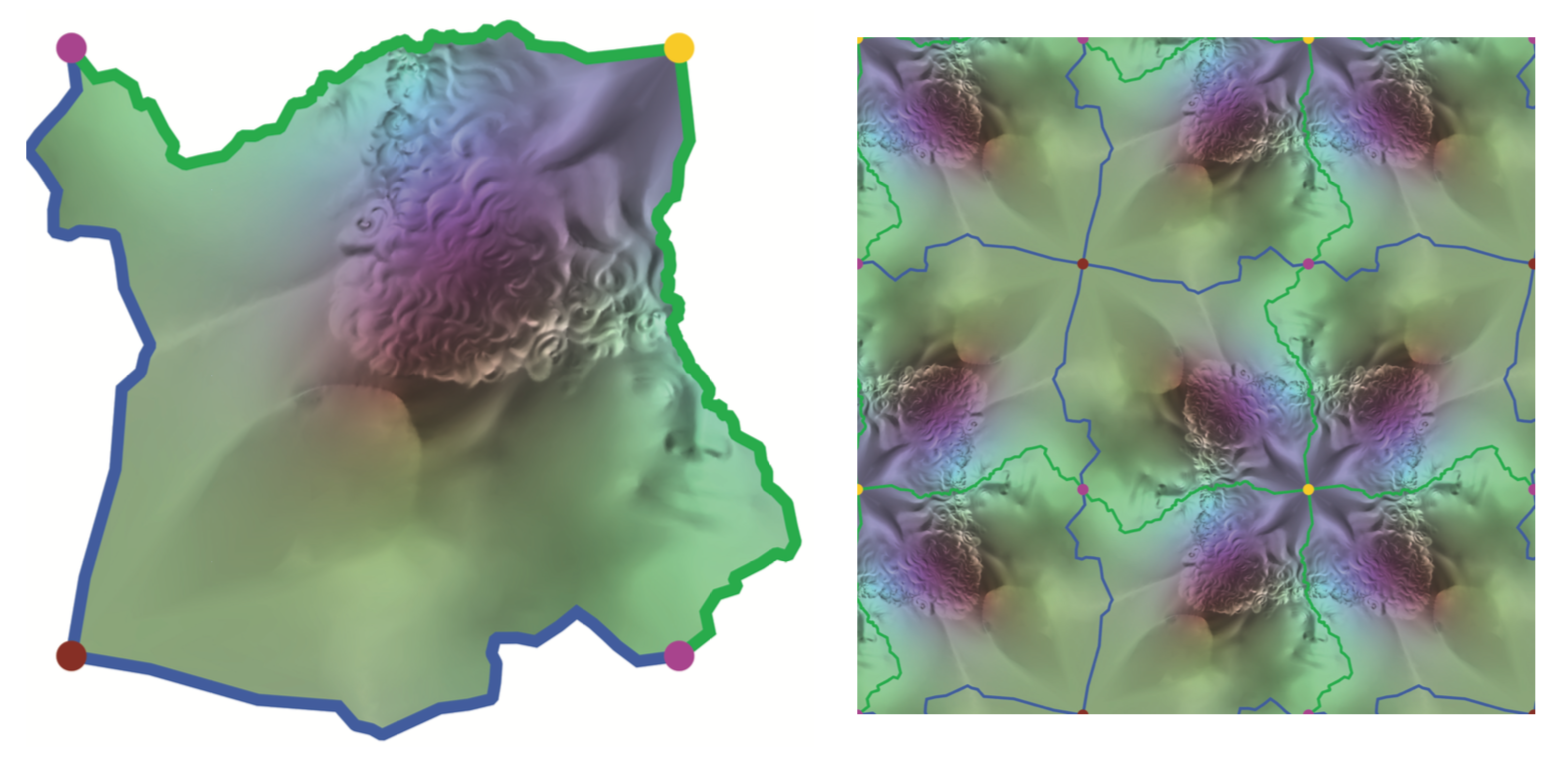
\includegraphics[width=\textwidth]{images/euc_orbifold}
\caption{}
\label{fig:tile}
\end{subfigure}
\begin{subfigure}[b]{0.5\textwidth}
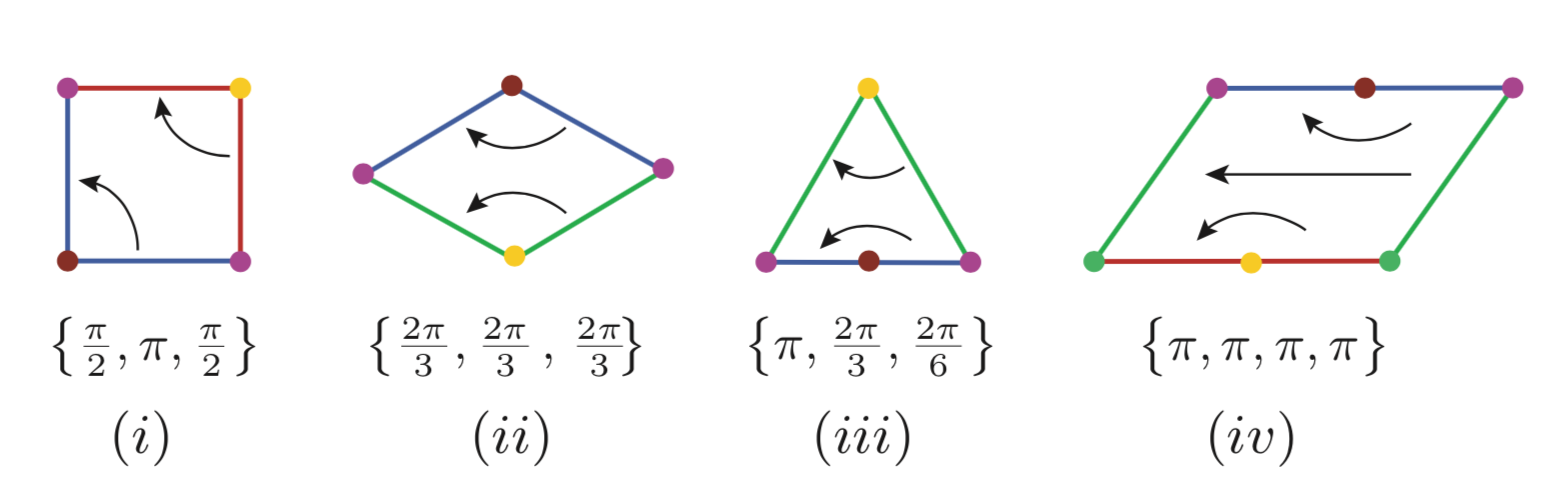
\includegraphics[width=\textwidth]{images/four_euc_orbifolds}
\caption{}
\label{fig:four-kinds}
\end{subfigure}
\caption{(a) Tiled 2d plane by one kind of orbfolds. (b) There are only four kinds of Euclidean orbifolds with spherical topology.}
\end{figure}

\subsubsection{Harmonic System with Rigid Constraints}

To get the parameterization, assume the singularities are $C$, we first find a single path that through all singularities and cut the mesh $M$ into a disk mesh $\bar{M}$. Some singularities will be split into two copies. We denote the new set of singularities as $\bar{C}$.

Each boundary vertex $v\not \in \bar{C}$ has a equivalent vertex $v'$, they are related be a rigid motion $R_{i'i}$.

The system to be solved is:

\begin{equation}
\begin{split}
&\sum_{v_j \in N(v_i)}w_{ij}(z_j - z_i) = 0, &v_i \in \bar{V}-\bar{B}\\
&\sum_{v_j \in N(v_i)}w_{ij}(z_j - z_i) + \sum_{v_j\in N(v_{i'})} w_{i'j}R_{i'i}(z_j - z_i')= 0, &v_i \in \bar{B} - \bar{C}\\
&z_i = z_i^0 , &v_i \in \bar{C}
\end{split}
\end{equation}

This system is full-rank, so it has a unique solution.

\subsubsection{Properties}

\textbf{Injectivity. }
By rotation around a singularity which doesn't have a equivalent vertex and by gluing, we will get a global parameterization of torus, see Fig.\ref{torus}. \cite{Gortler:2006:DOM:1133946.1648437} had proven that in this case, the result is an embedding. 

\begin{figure}
\centering
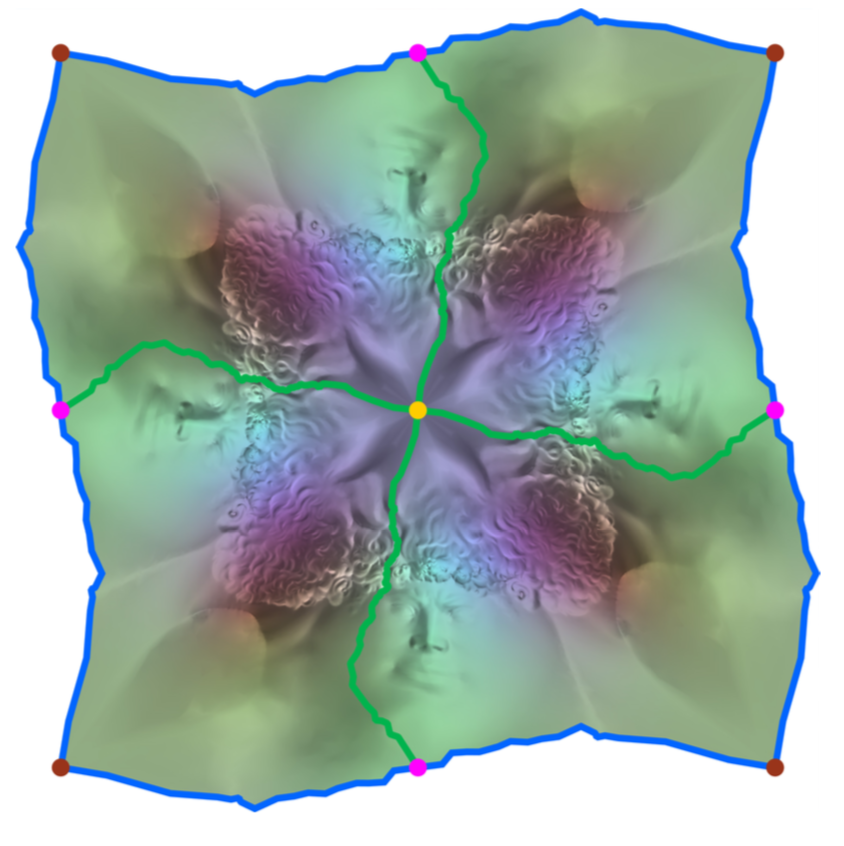
\includegraphics[width=0.3\textwidth]{images/torus}
\caption{Proof of injectivity.}
\label{torus}
\end{figure}


\textbf{Conformality.} 
If we choose cotangent weights, the map is a minimizer of the conformal energy functional defined on bijective maps from $M$ to its corresponding orbifold:
$$ E_C(\Phi) = E_D(\Phi) - Area(\Phi)$$
where $$E_D(\Phi) = \frac{1}{2}\int_M |\Delta \Phi|^2 $$

The algorithm is a linear method to compute conformal map of sphere. By double cover technique, this means we get a linear method to compute conformal map of disk.


\subsection{Hyperbolic Orbifold and Spherical Orbifold Tutte Embeddings}

This subsection, I will review \cite{Aigerman:2016:HOT:2980179.2982412} and \cite{Aigerman:2017:SOT:3072959.3073615}
These two paper is extension the idea of \cite{Aigerman:2015:OTE:2816795.2818099} into hyperbolic geometry and spherical geometry.

The same as Euclidean orbifolds, hyperbolic and spherical orbifolds are also tiled space, but one is of the hyperbolic space $\mathbb{H}^2$ and the other one is of the spherical space $\mathbb{S}^2$. In these two paper, we choose  Poincar\'e disk and standard sphere as the underlying space. See Fig.\ref{fig:hs}.

\begin{figure}
\begin{subfigure}[b]{\textwidth}
\centering
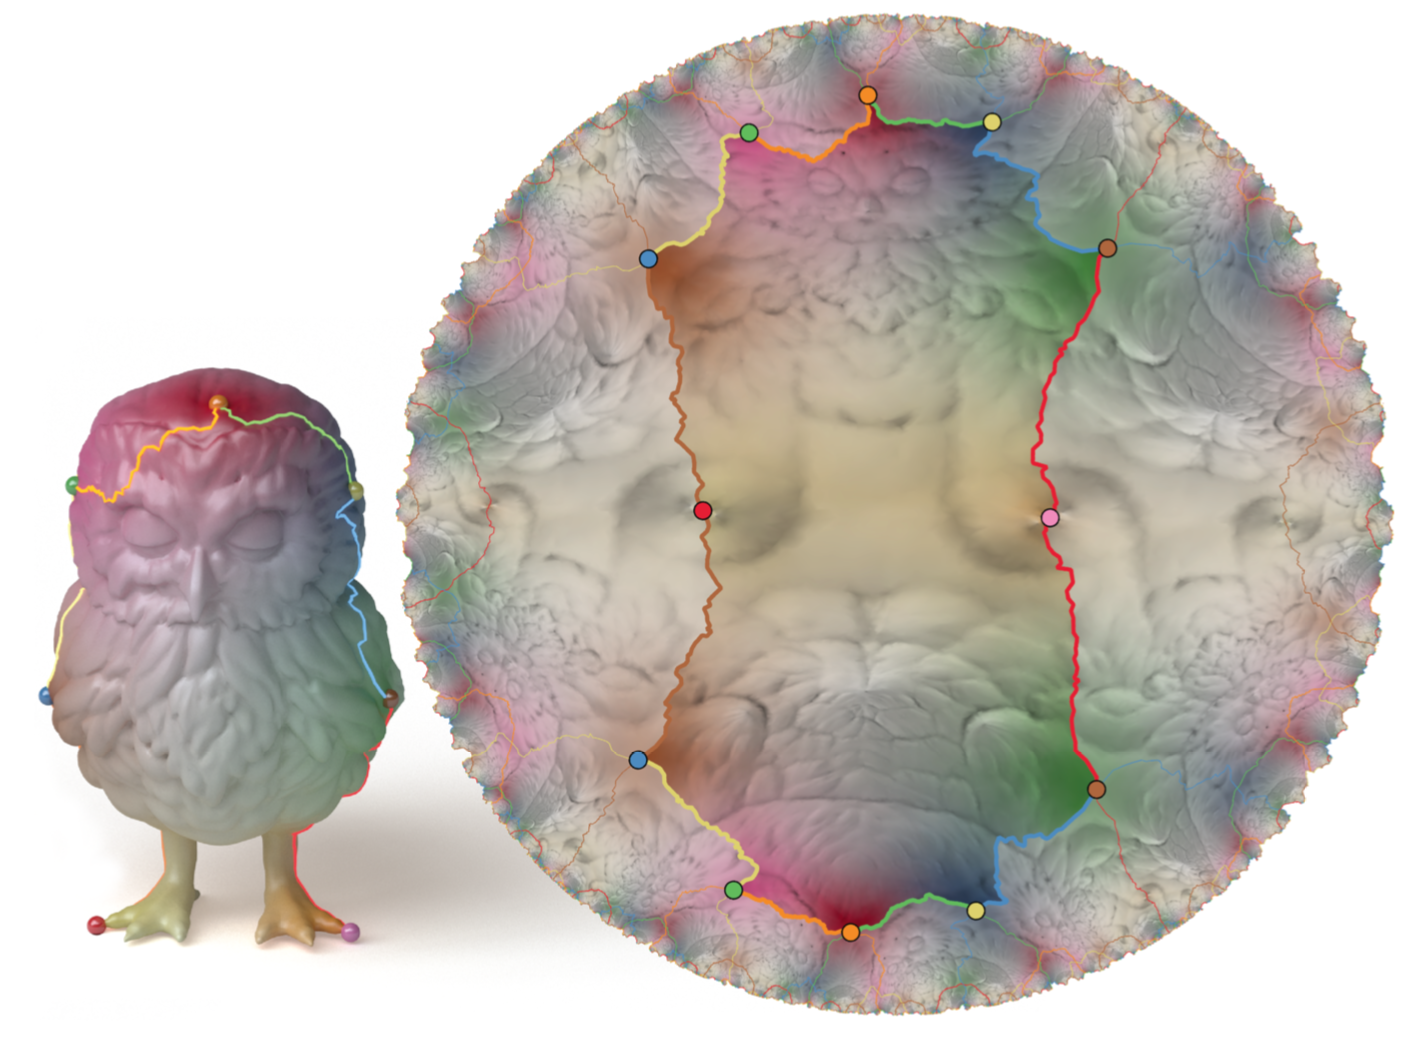
\includegraphics[width = 0.25\textwidth]{images/hyperbolic}
\caption{}
\end{subfigure}
\begin{subfigure}[b]{\textwidth}
\centering
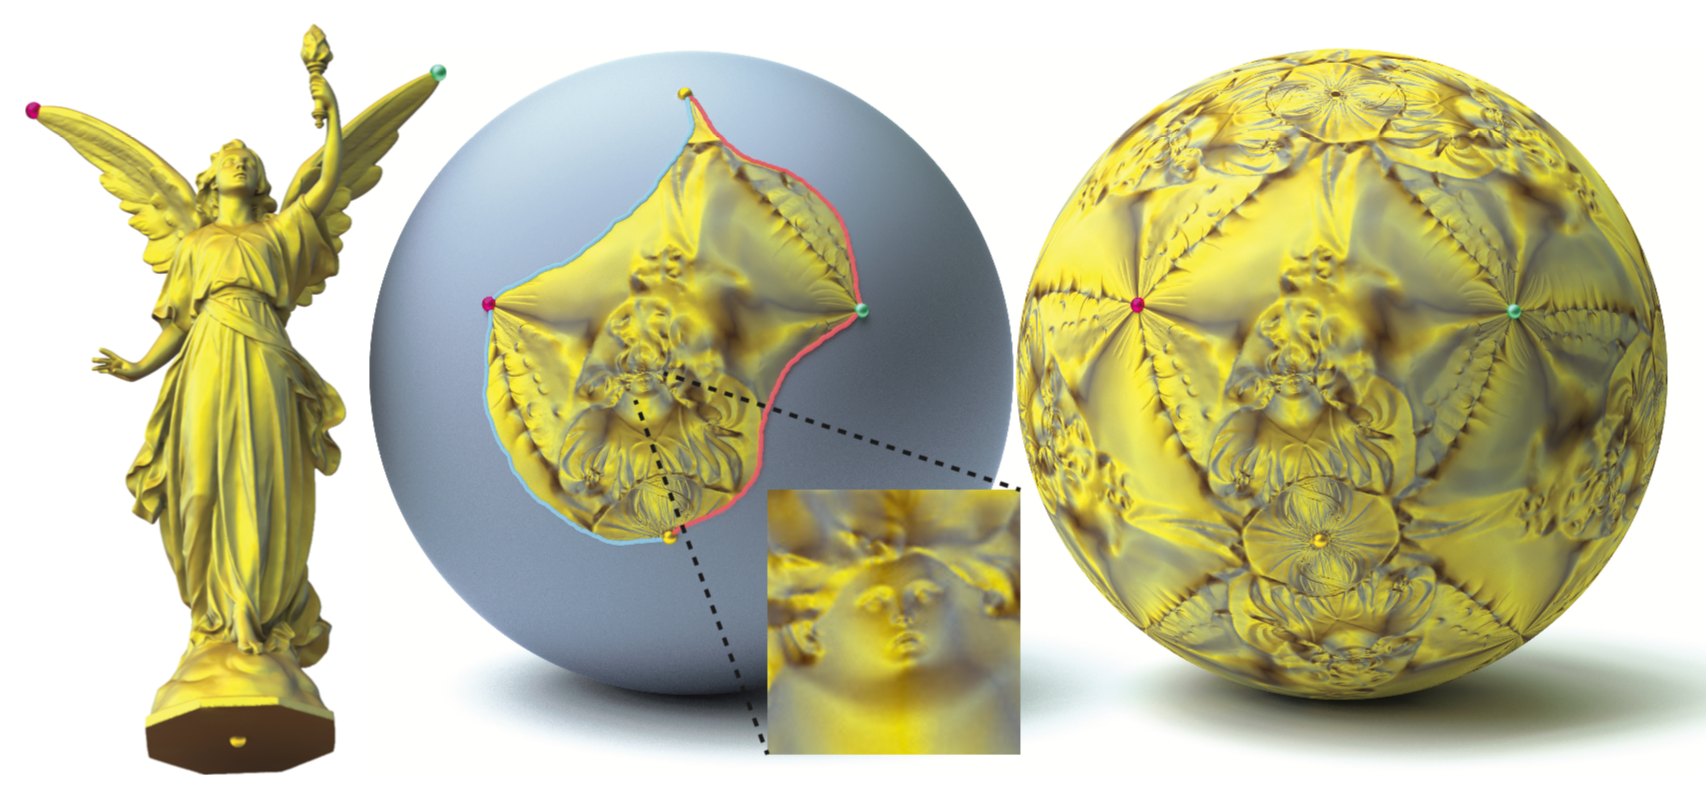
\includegraphics[width = 0.4\textwidth]{images/spherical}
\caption{}
\end{subfigure}
\caption{(a) Hyperbolic orbifold.  (b) Spherical orbfold.}
\label{fig:hs}
\end{figure}




\subsubsection{Non-linear Optimization}

Tutte embedding's solution is a global minimizer of some Dirichlet energy:
\begin{equation}
E(\Phi) = \frac{1}{2}\sum_{(i,j)\in E} w_{ij} d(z_i, z_j)^2
\end{equation}
where $d$ is distance in the corresponding space: hyperbolic distance or spherical distance.

Same as euclidean orbifold, after cutted into disk, equivalent vertex pairs should satisfy rigid constraints. Hyperbolic orbifolds are constrained by hyperbolic isometries, namely, Mobius transformations. Spherical orbifolds are constrained by shperical isometries, namely, 3d rotations around the sphere center.

So, to get the parameterization, we need to solve the following optimization:
\begin{equation}
\begin{split}
&\min_{\Phi} E(\Phi),&\\
s.t \ \ \ &z_i = m_{i'i}(z_{i'}), &v_i \in \bar{B} - \bar{C}\\
 &z_i = z_i^0, &v_i \in \bar{C}\\
\end{split}
\end{equation}

By the knowledge of hyperbolic geometry and spherical geometry, the distance between two points has explicit expression, and the first-order derivative is easy to compute as well. So we can use first-order optimization algorithm to minimize the energy.

\subsection{Properties}

\textbf{Injectivity.}
The proof of injectivity is based on the following theorem:
\begin{theorem}
$$grad_{z_i}E(\Phi) = -\sum_{j\in N_i} w_{ij} Exp^{-1}_{z_i}(z_j)$$
\end{theorem}
where $Exp_{p}: T_p \rightarrow M$ is exponential map on the Riemannian manifolds $\mathbb{H}^2$ or $\mathbb{S}^2$.

This means when $grad_{z_i}E(\Phi) = 0$, each $z_i$ is some strict Euclidean convex combination of its neighbors, which leads to the injectivity.


\section{Harmonic Global Parametrization with Rational Holonomy}

\cite{Bright:2017:HGP:3072959.3073646} is a deeper generalization of Euclidean orbifolds. This paper solved the limitation of euclidean orbifold on the number of types and the algorithm can be applied to any topology.  This algorithm is based on complex analysis and Riemann surfaces. 

The parameterization will generate a kind of Riemann surface structure called q-fold branch covers, instead of orbifolds. But the same as Euclidean orbifold, the transformations are still rigid motions in Euclidean space.

\subsection{Harmonic System}

The system we want to solve is still harmonic. That is, the interior vertices are co-closed and all faces are closed. 

Assume the singularities are $C$, the boundary components are $B$, we need to cut the mesh $S$ into a disk $S_C$, the slice form a graph $G_C$, which cut through all singularities and boundary components.  Each edge in $G_C$ will be split into two copies, and each vertex in $G_C$ will be split into at least two copies. 

For each pair of equivalent edges $e_{ij}^a, e_{ij}^b$, we need to maintain the rigid constraint: 
\begin{equation}
z^a_{j}-z^a_i=e^{i\frac{2\pi r_{ij}}{q} (z^b_j-z^b_j)}, e_{ij}\in G_C
\end{equation}
where $r_{ij} \in \{0,1,...,q-1\}.$

This is where rational holonomy comes from.

\subsection{Q-fold Branch Cover}

Under these constraints, $S_C$ forms a basic tile of a q-fold branch cover $S_q$ of $M$.

q-fold is determined by the rotation angles $\frac{2\pi k_i}{q}$ of singularities and the rotation angles $\frac{2\pi l_i}{q}$ of boundary components.

The choice of $l,k$ must satisfy the following Gauss-Bonet theorem for q-fold branch cover:
\begin{theorem}
$$q|C|- \sum_{v_i \in C} k_i + \sum_{j=1 }^m l_j =q(2-2g -m).$$
\end{theorem}

\begin{figure}
\begin{subfigure}[b]{0.7\textwidth}
\centering
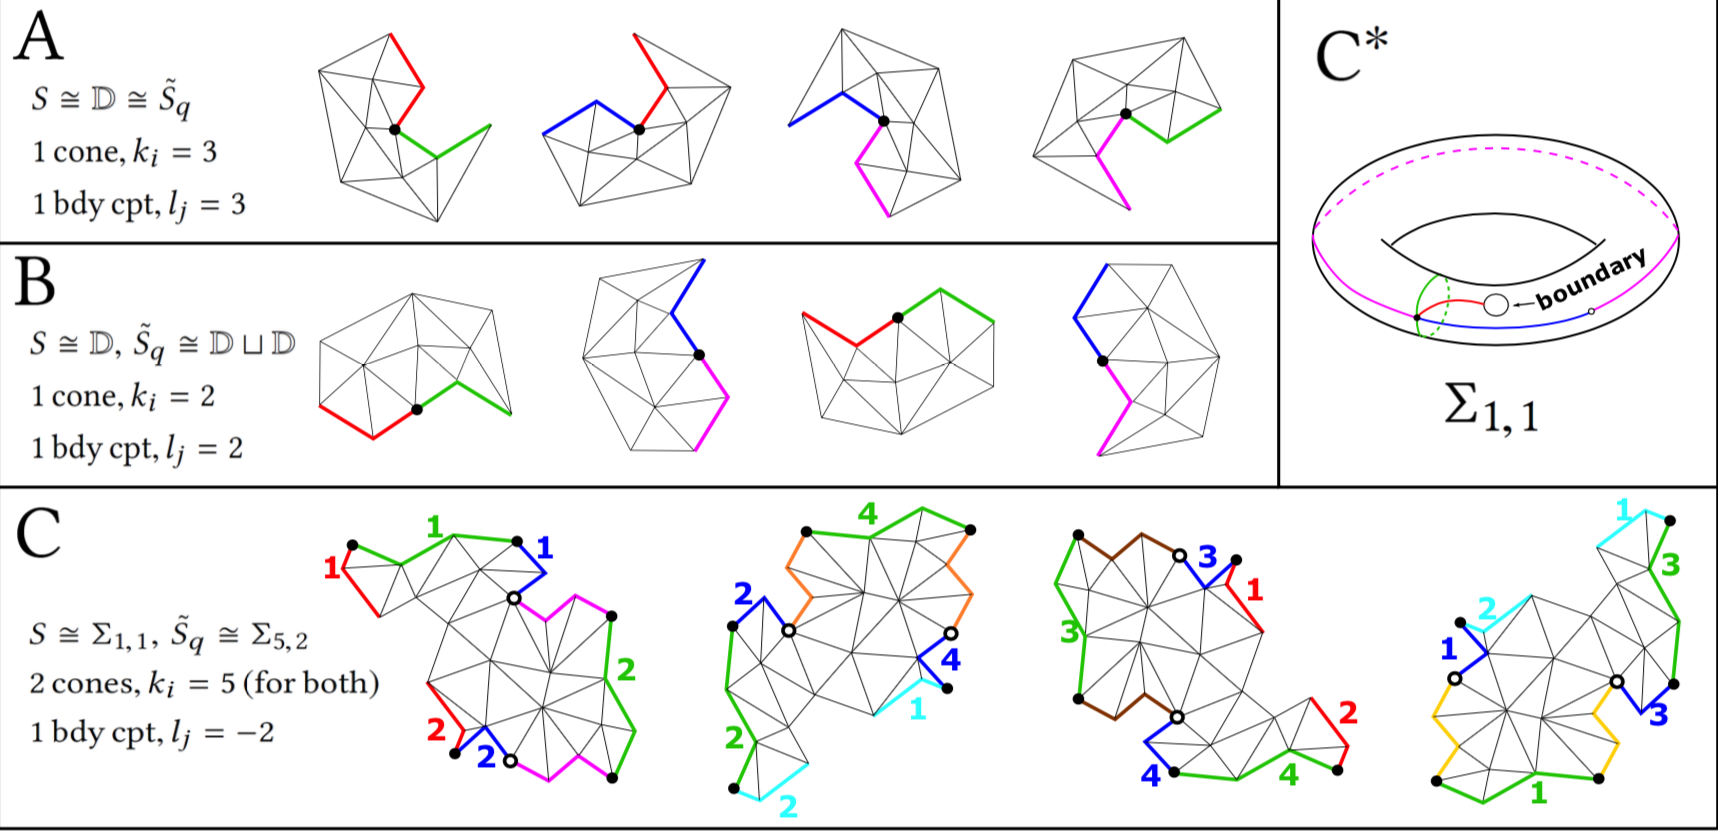
\includegraphics[width=\textwidth]{images/q-folds}
\end{subfigure}
\begin{subfigure}[b]{0.2\textwidth}
\centering
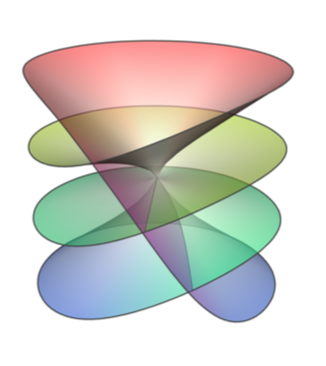
\includegraphics[width=\textwidth]{images/q-fold}
\end{subfigure}
\caption{Examples of q-fold branch covers.}
\label{fig:q-fold}
\end{figure}

Here are some examples of q-fold branch covers in Fig.\ref{fig:q-fold}. The right part is the visualization of A in the left part. It's a Riemann surface. The behavior at that sigularity is the same as $f = z^{1/4}$.

\subsection{Convex Optimization}

The algorithm solves the following convex optimization:
\begin{equation}
\begin{split}
&\min_{z_i} ||L(z)||^2&\\
s.t\  \ \ \ \  & z^a_{j}-z^a_i=e^{i\frac{2\pi r_{ij}}{q} (z^b_j-z^b_j)}, &e_{ij}\in G_C\\
&Re(f_z \frac{|\tilde{f}_z^j|}{\tilde{f}_z^j}) - |f_{\bar{z}}| > \epsilon , &t_j \in F_{cb}
\end{split}
\end{equation}

The second constraints is on all boundary faces. As discussed in \cite{Gortler:2006:DOM:1133946.1648437}, the behavior of interior is determined by boundary. This kind of constraints is from \cite{Lipman:2012:BDM:2185520.2185604} and \cite{Chen:2015:BDH:2809654.2766989}. The purpose of this is to add bound on the conformal distorsion, while maintain the convexity of feasible area. So the problem can be solved by convex optimization. 



\subsection{Properties}

The author proved the locally injectivity by Gauss-Bonet theorem, by showing that every inner vertex is a wheel.  The locally injectivities means that each vertex has a neighborhood on which the map is injective but not global. Example is showned in Fig.\ref{fig:locally-injectivity}

\begin{figure}
\centering
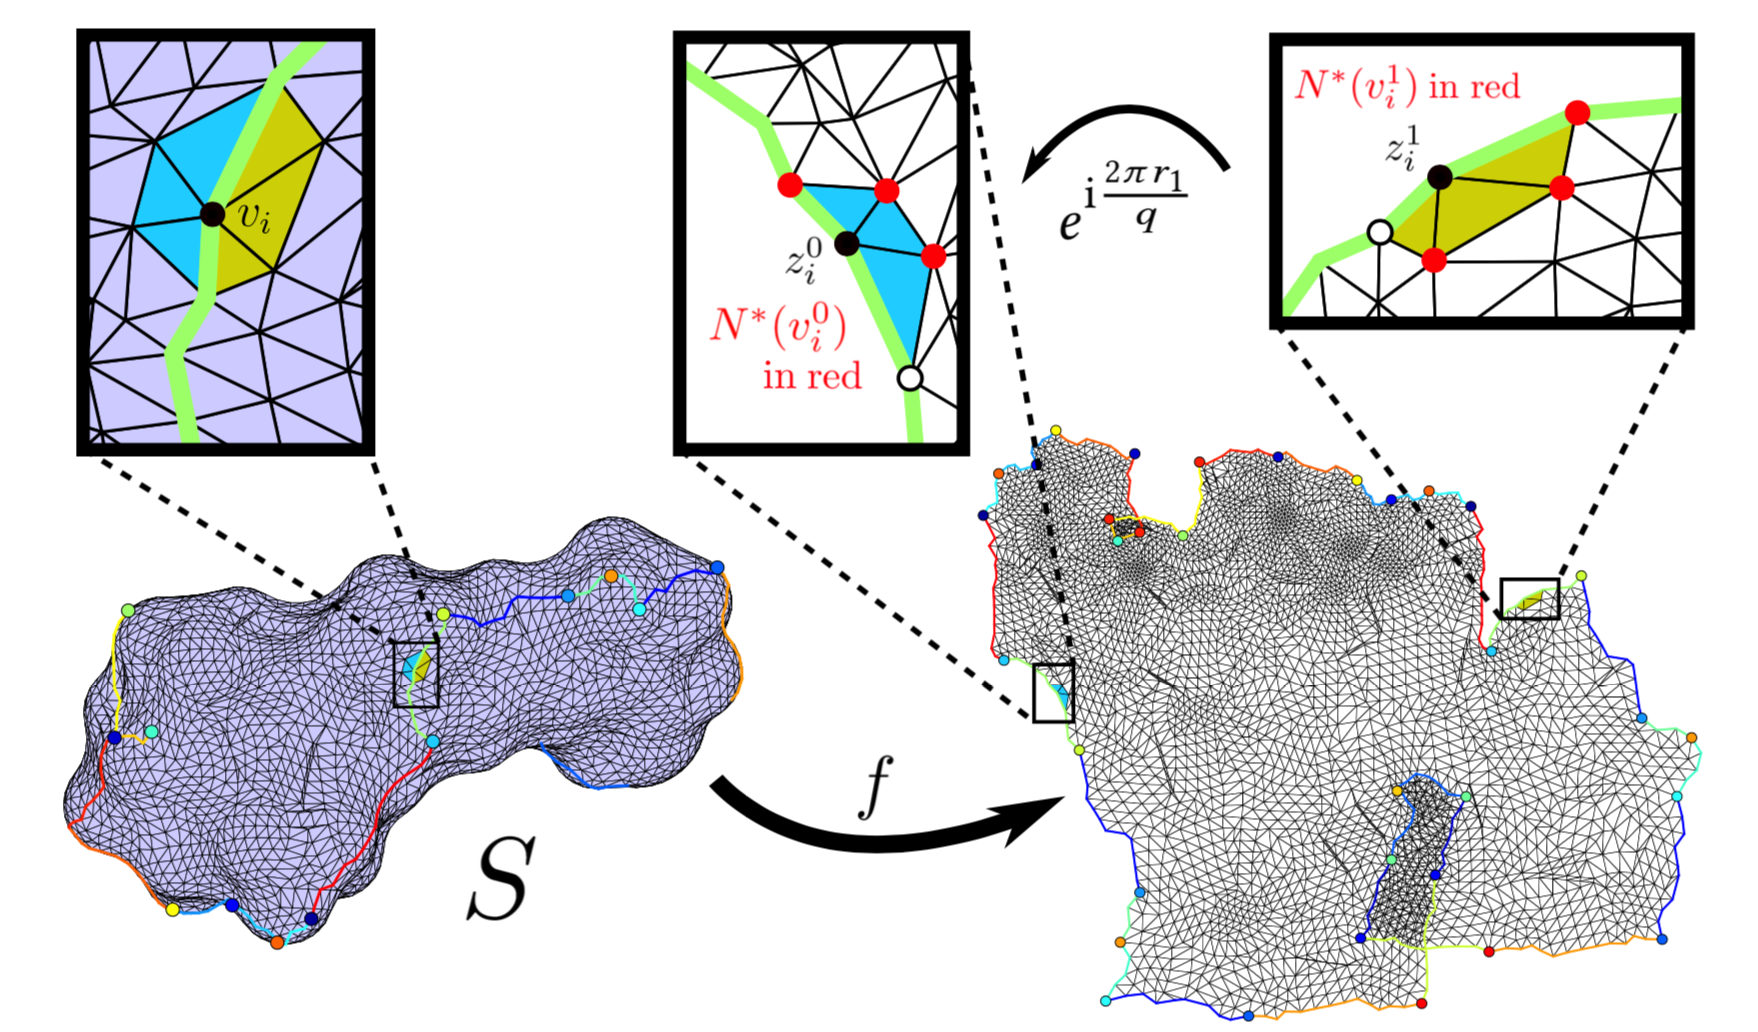
\includegraphics[width=0.7\textwidth]{images/locally}
\caption{Locally injective map.}
\label{fig:locally-injectivity}
\end{figure}


\section{Boundary First Flattening }
\cite{1704.06873} proposed a linear method to compute conformal parameterization of surfaces from the view of differential geometry. This paper also provided a method to compute global parameterization after cutting. The tools includes Poisson equation, Cherrier formula and Poincar\'e-Steklov operators.

The pipeline of BFF is as follows:
1. Define boundary data. 
2. Integrate boundary data to a closed loop.
3. Extend the exterior loop into the interior conformally.

\subsection{Poisson Equation}

In continuous setting, a conformal map $f$ between any two surfaces satisfy:
\begin{equation}
\begin{split}
\Delta u = K - e^{2u} \tilde{K} \ \ \ &on\ &M\,\\
\frac{\partial u}{\partial n} = k - e^{u}\tilde{k} \ \ \ &on\     &\partial M
\end{split}
\end{equation}
where $u$ is conformal factor, $K$,$\tilde{K}$ are Gauss curvature of the source surface and  the target surface, $k, \tilde{k}$ is geodesic curvature of the source surface and the target surface.

These two equations can be converted into the form of curvature densities:
\begin{equation}
\begin{split}
\Delta udA = KdA - \tilde{K}d\tilde{A}  \ \ \ &on\ &M\,\\
\frac{\partial u}{\partial n} ds = kds - \tilde{k} d\tilde{s}\ \ \ &on\     &\partial M
\end{split}
\label{eq:linear}
\end{equation}

This is where the linearity appears.

Given a discrete mesh $M = (V, E, F)$, integrate Eq.\ref{eq:linear} on dual cells, we get

\begin{equation}
\begin{split}
Au &=   \Omega - \tilde\Omega\  &on\  Int\  M\\
h &= k - \title{k}\ \  &on\ \partial M 
\end{split}
\label{eq:poisson}
\end{equation}
where A is the cotangent Laplacian matrix.
And $\Omega_i = 2\pi - \sum_{ijk \in F}\theta_i^{jk}$ defined on interior vertices, $k_i = \pi - \sum_{ijk \in F}\theta_i^{jk}$ defined on boundary vertices.

Combine them we can get 
\begin{equation}
\left(\begin{matrix}
A_{II} & A_{IB}\\
A_{BI} & A_{BB}
\end{matrix}\right) u
= \left(\begin{matrix}
\Omega - \tilde{\Omega}\\
h\end{matrix}\right)
\label{eq:relation}
\end{equation}

Eq.\ref{eq:poisson} is a discrete Poisson equation. By Eq.\ref{eq:relation} we can convert between Riemman boundary data and Dirichlet boundary data. So we can convert between boundary $\tilde{k}$ and boundary $u$.

This is the core part of the BBF. With this insight, we can either define boundary $u$ or boundary $\tilde{k}$ and get the other.

That's why the algorihtm is called "boundary first".

\subsection{Integral of Curve}
$u$ is related with metric (i.e edge length) of the mesh. The same as \cite{Springborn:2008:CET:1360612.1360676}, the edge length here is defined as $\tilde{l}_{ij} = l_{ij}e^{\frac{u_i + u_j}{2}}$, where $l$ is actual Euclidean length of the mesh. And the metric $\tilde{l}$ is said to be conformally equivalent with $l$. The theories above is actually construct on this edge length definition, since the integral on dual cells need the definition of length
.

Knowing the boundary $u$ and $\tilde{k}$, it is reasonable that we can intergrate to get a loop, but the reality is showned in Fig.\ref{fig:loop}.

\begin{figure}
\centering
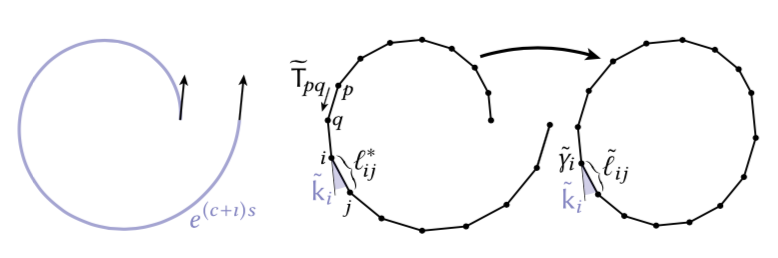
\includegraphics[width=0.5\textwidth]{images/loop}
\caption{We need to modify the lengths of segments a little to get a closed loop}
\label{fig:loop}
\end{figure}

So we first compute cumulative angles as $ \phi_p = \sum_{i = 1}^{p-1}\tilde{k}_i$. And define tengent vectors $T_{ij} = (\cos \phi_i, \sin \phi_i)$. Then we solve the optimization problem:
\begin{equation}
\begin{split}
&\min_{l^*} \frac{1}{2}\sum_{ij \in \partial M}l_i^{-1} |l^*_{ij} - \tilde{l_{ij}}|^2\\
s.t  \ \ \ \ &\sum_{ij\in \partial M}l^*_{ij}T_{ij} = 0.
\end{split}
\end{equation}
where $l_i = \frac{l_{ki} + l_{ij}}{2}$ is the dual edge length.

This idea is from global differential geometry on how we integral the curvature of a loop to the position of the loop.

\subsection{Conformal Extension}
A conformal map must be a harmonic map, so one choice is to extend into interior by harmonic map, that is, Tutte embedding with cotangent weights.

But due to the discretization, a lot of errors occur, so another choice is that we extend only one component $a$ by harmonic map, and for the other component $b$ we choose to minimize the conformal energy. This is done by apply Hilbert transform operator on $a$, which is defined as:
\begin{equation}
(Ha)_j = \frac{1}{2} (a_k - a_i) 
\end{equation}
where ijk are three consecutive vertices on the boundary.
Then we solve the Poisson equition:
\begin{equation}
\begin{split}
Ab &=   0\  &on\  Int\  M\\
\frac{\partial b }{\partial n} &= Ha\ \  &on\ \partial M 
\end{split}
\end{equation}
This is called harmonic conjugation.


\begin{figure}
\centering
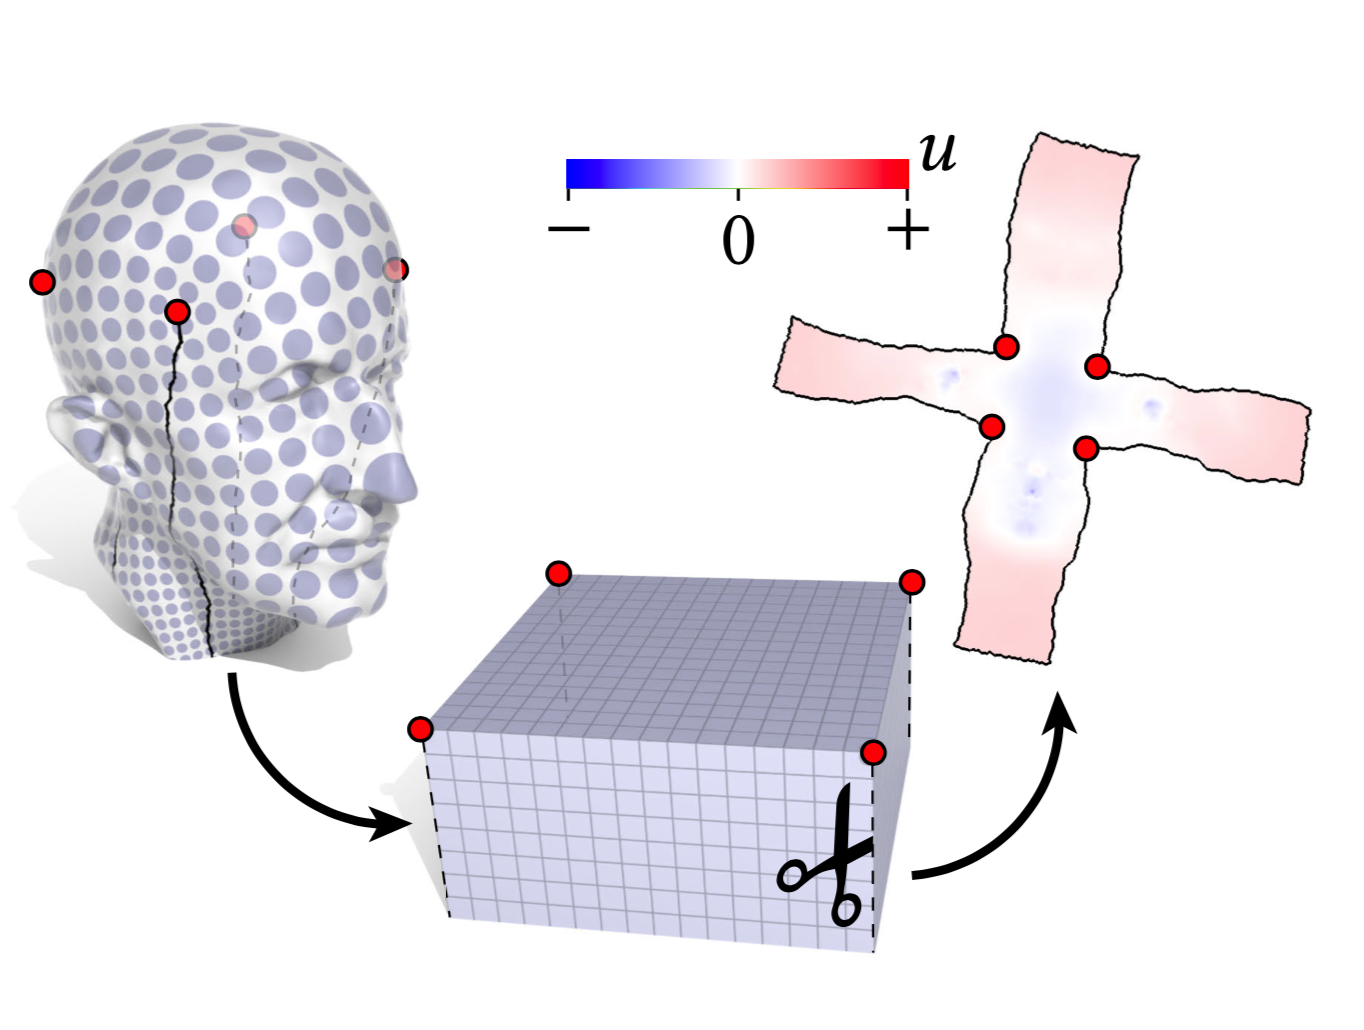
\includegraphics[width=0.5\textwidth]{images/cone}
\caption{Cone parameterization}
\label{fig:cone}
\end{figure}


\subsection{Global Parameterization}
BFF can be applied to get global parameterization of cone surfaces. As before, we cut through all cones to get a disk. We want to get a global parameterization of the cutted mesh.

To get boundary $u$ and $\tilde{k}$, before cutting, we solve Eq.\ref{eq:poisson} on $M$ to get $u$. Then we cut the mesh into $\bar M$ and maintain $u$ of the boundary. Using this $u$ as input, we use normal BFF algorithm to get the parameterization. Note that when optimize closed curve condition, we assign only one variable to each pair of equivalent edges. By this new constraint, we know the result is a global parameterization. The example is showned in \ref{fig:cone}.







 




\bibliographystyle{apalike}
\bibliography{sample}


\end{document}